\documentclass[journal,10pt,onecolumn,compsoc]{IEEEtran} 
    \usepackage[margin=0.75in]{geometry} 
    \usepackage{pdfpages} 
    \usepackage{graphicx} 
    

    \usepackage{tikz}
    \usetikzlibrary{shapes,arrows}
    \tikzstyle{block} = [rectangle, draw, fill=blue!20, 
    text width=5.5em, text centered, rounded corners, minimum height=4em]
    \tikzstyle{subblock} = [rectangle, draw, fill=blue!20, 
    text width=7em, text centered, rounded corners, minimum height=2em]
    \tikzstyle{datablock} = [rectangle, draw, fill=red!20, 
    text width=7em, text centered, rounded corners, minimum height=2em]
    \tikzstyle{line} = [draw, -latex']  
   
    \newenvironment{paddedtikzpicture}{\vspace*{0.5cm}
    \begin{center}\begin{tikzpicture}}
    {\
    \end{tikzpicture}\end{center}
    } 
    \usepackage[english]{babel}
    \usepackage{graphicx}
    \usepackage{url}
    \usepackage{setspace}
    \usepackage{geometry}
    \usepackage{hyperref}
    \usepackage{caption} 
    \usepackage{float}
    \usepackage{pgfgantt}
    \usepackage{rotating} 
    \usepackage{ragged2e} % provides \RaggedLeft
    \hypersetup{
        colorlinks,
        citecolor=black,
        filecolor=black,
        linkcolor=black,
        urlcolor=black
    }
    \geometry{textheight=9.5in, textwidth=7in}
    
    % 1. Fill in these details
    \def \CapstoneTeamName{		The Dream Team}
    \def \CapstoneTeamNumber{		57}
    \def \GroupMemberOne{			Daniel Schroeder}
    \def \GroupMemberTwo{			Aubrey Thenell}
    \def \GroupMemberThree{			Parker Bruni}
    \def \CapstoneProjectName{		A Scalable Web Application Framework for Monitoring Energy Usage on Campus  }
    \def \CapstoneSponsorCompany{	Oregon State Office of Sustainability}
    \def \CapstoneSponsorPerson{		Jack Woods}
    
    % 2. Uncomment the appropriate line below so that the document type works
    \def \DocType{		%Problem Statement
            %Requirements Document
            %Technology Review
            Design Document
            %Progress Report
            }
          
    \newcommand{\NameSigPair}[1]{\par
    \makebox[2.75in][r]{#1} \hfil 	\makebox[3.25in]{\makebox[2.25in]{\hrulefill} \hfill		\makebox[.75in]{\hrulefill}}
    \par\vspace{-12pt} \textit{\tiny\noindent
    \makebox[2.75in]{} \hfil		\makebox[3.25in]{\makebox[2.25in][r]{Signature} \hfill	\makebox[.75in][r]{Date}}}}
    % 3. If the document is not to be signed, uncomment the RENEWcommand below
    %\renewcommand{\NameSigPair}[1]{#1}
    
    %%%%%%%%%%%%%%%%%%%%%%%%%%%%%%%%%%%%%%%
    \title{Design Document for: \linebreak Scalable Web Application Framework for Monitoring Energy Usage on Campus}
    \author{Daniel Schroeder, Aubrey Thenell, Parker Bruni}
    \date{\today}
    
    \begin{document}
    \maketitle
    \vspace{2cm}
    \begin{center}
    \noindent \textbf{Abstract} \\
                \indent 
                
                
    \end{center}         
    
    \newpage
    \pagenumbering{arabic}
    \tableofcontents
    % 7. uncomment this (if applicable). Consider adding a page break.
    %\listoffigures
    %\listoftables
    \clearpage
    
    % 8. now you write!
    \section{Introduction}
    \subsection{Purpose}
    Identify the purpose of this SDD and its intended audience. (e.g. “This software
    design document describes the architecture and system design of XX. ….”).
    \subsection{Scope}
    Provide a description and scope of the software and explain the goals, objectives and
    benefits of your project. This will provide the basis for the brief description of your
    product.
    \subsection{Overview}
    Oregon State University is constantly making strides to reduce its carbon footprint and reduce its energy consumption. There is a carbon neutrality goal for 2025 where the university is trying to generate as much energy as it uses and have a net carbon footprint of 0. Our web application aims to monitor the energy use of buildings on campus in order to create a visual representation of each building's consumption and incentivize people to monitor their consumption habits and reduce the campus's overall consumption.
    Our web application will resemble an administrative dashboard that has charts and graphs of energy use over time for individual buildings and subgroups of buildings on Oregon State's campus. 
    Our application will have a series of public facing pages that show general data use for all the buildings on campus that have AcquiSuites as well as user generated stories of personalized dashboards. Each page will be a grid-based dashboard with personalized blocks for displaying data through time-series charts or graphs. A user will be able to add different blocks to their pages to create a unique dashboard for their own unique interests and subsets of buildings. An example of this would be a page designated to only residence halls where each block shows a usage over time graph for energy consumption of each residence hall. Users will be able to apply date filters to their blocks to generate different data sets and more explicit visualizations.
    Our web application will be constructed using a MEAN Stack framework hosted on AWS. Our application will have a MongoDB database server and a Node.js application server hosted on a single virtual EC2 instance to make deployment easy and reliable.
    \subsection{Reference Material}
    List any documents, if any, which were used as sources of information for the test plan.
    \subsection{Definitions and Acronyms}
    Provide definitions of all terms, acronyms, and abbreviations that might exist to
    properly interpret the SDD. These definitions should be items used in the SDD that
    are most likely not known to the audience. 
    \begin{itemize}
        \item \textbf{Dashboard:}
            A grid-based information management tool for visually tracking and displaying metrics and data through graphs and charts.
        \item \textbf{Block:} 
            An individual graph or chart depicting time-series data.
        \item \textbf{Page:} 
            A dashboard of different blocks. 
        \item \textbf{Story:} 
            A user generated collection of pages. 
        \item \textbf{MEAN Stack:} 
            An acronym used to define a full stack application engineered from the MongoDB, Express.js, Angular.js, and Node.js frameworks. 
        \item \textbf{Bootstrap:} 
            Bootstrap CSS is a front-end framework that uses component templates to easily generate different HTML elements like buttons, navigation, or forms. 
        \item \textbf{OAuth 2.0:} 
            OAuth 2.0 is an authorization protocol that grants authentication through tokens rather than credentials. 
        \item \textbf{Filter:} 
            Filters are essentially parameters for fetching data from that constrain the subset of data being received to the specifications of the filter parameters (i.e. a date range). 
        \item \textbf{D3:} 
            D3.js is a visualization framework that appends charts and graphs to DOM elements on a webpage. 
        \item \textbf{AcquiSuite:} 
            AcquiSuites are data acquisition servers made by a company called Obvius that post building meter data to a designated IP address.
        \item \textbf{AWS:} 
            AWS is an acronym for Amazon Web Services which offers reliable cloud computing services for building and hosting web applications.
    \end{itemize}
    \section{System Overview}
    \textit{Give a general description of the functionality, context and design of your project.
    Provide any background information if necessary.} 
    Oregon State University is constantly making strides to reduce its carbon footprint and reduce its energy consumption. There is a carbon neutrality goal for 2025 where the university is trying to generate as much energy as it uses and have a net carbon footprint of 0. Our web application aims to monitor the energy use of buildings on campus in order to create a visual representation of each building's consumption and incentivize people to monitor their consumption habits and reduce the campus's overall consumption.\\
    Our web application will resemble an administrative dashboard that has charts and graphs of energy use over time for individual buildings and subgroups of buildings on Oregon State's campus.\\
    Our application will have a series of public facing pages that show general data use for all the buildings on campus that have AcquiSuites as well as user generated stories of personalized dashboards. Each page will be a grid-based dashboard with personalized blocks for displaying data through time-series charts or graphs. A user will be able to add different blocks to their pages to create a unique dashboard for their own unique interests and subsets of buildings. An example of this would be a page designated to only residence halls where each block shows a usage over time graph for energy consumption of each residence hall. Users will be able to apply date filters to their blocks to generate different data sets and more explicit visualizations.\\
    Our web application will be constructed using a MEAN Stack framework hosted on AWS. Our application will have a MongoDB database server and a Node.js application server hosted on a single virtual EC2 instance to make deployment easy and reliable.
    \section{System Architecture}
    \subsection{Architectural Design}
    Develop a modular program structure and explain the relationships between the
    modules to achieve the complete functionality of the system. This is a high level
    overview of how responsibilities of the system were partitioned and then assigned to
    subsystems. Identify each high level subsystem and the roles or responsibilities
    assigned to it. Describe how these subsystems collaborate with each other in order to
    achieve the desired functionality. Don’t go into too much detail about the individual
    subsystems. The main purpose is to gain a general understanding of how and why
    the system was decomposed, and how the individual parts work together. Provide a
    diagram showing the major subsystems and data repositories and their
    interconnections. Describe the diagram if required. 

    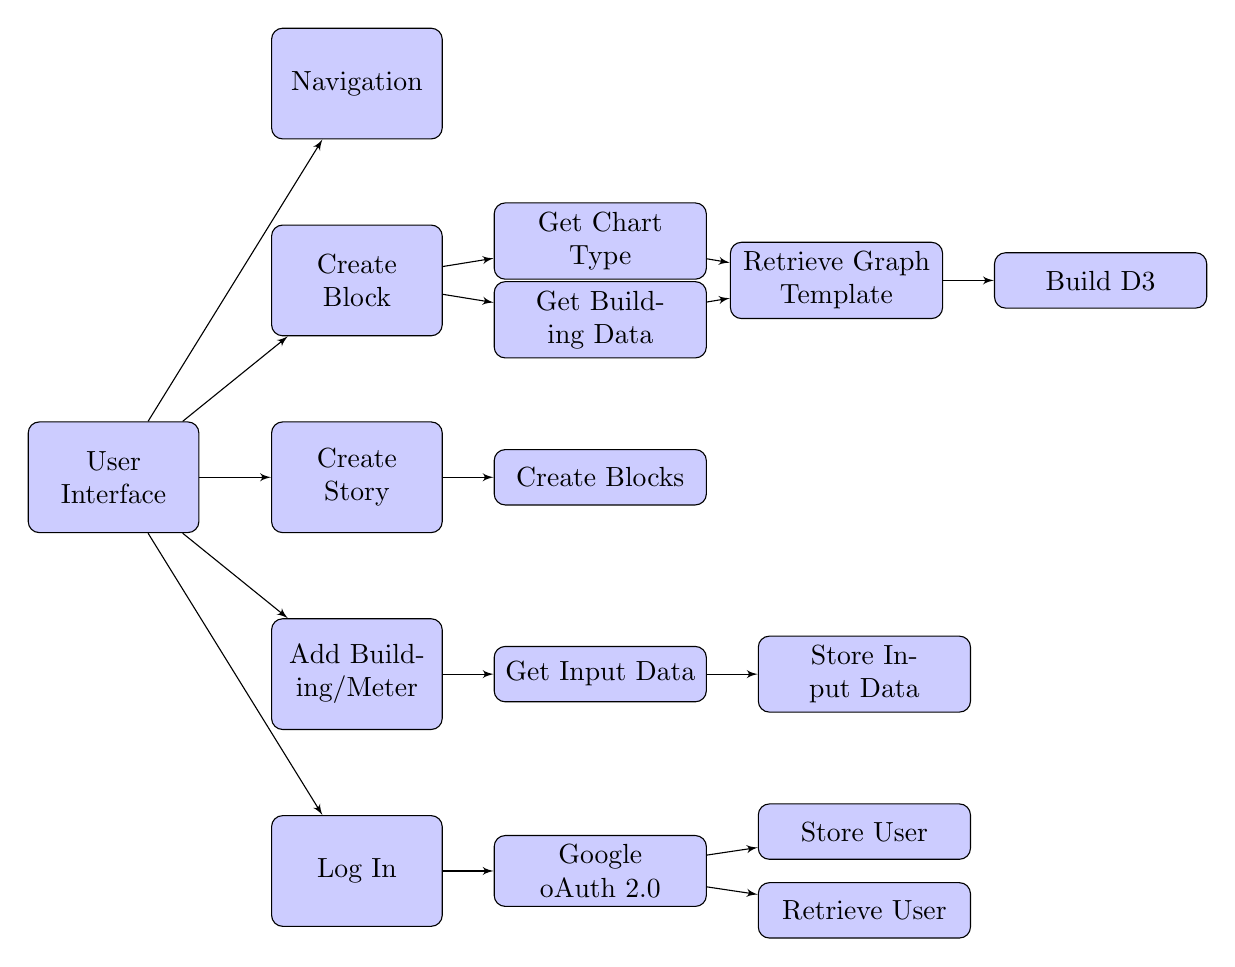
\begin{tikzpicture}[node distance = 2cm, auto]
        % Place nodes
        \node (ui)[block] {User Interface}; 
        \path (ui.east)+(2,5) node (nav) [block] {Navigation}; 
        \path [line] (ui) -- (nav);
        \path (ui.east)+(2,2.5) node (block) [block] {Create Block}; 
        \path [line] (ui) -- (block);
        \path (ui.east)+(2,0) node (story) [block] {Create Story}; 
        \path [line] (ui) -- (story);
        \path (ui.east)+(2,-2.5) node (add) [block] {Add Building/Meter};
        \path [line] (ui) -- (add);
        \path (ui.east)+(2,-5) node (log) [block] {Log In}; 
        \path [line] (ui) -- (log);
        
        %Create Block
        \path (block.east)+(2,0.5) node (ctype) [subblock] {Get Chart Type};
        \path [line] (block) -- (ctype);
        \path (block.east)+(2,-0.5) node (bdata)[subblock] {Get Building Data};
        \path [line] (block) -- (bdata); 
        \path (block.east)+(5,0) node (template)[subblock] {Retrieve Graph Template}; 
        \path [line] (bdata) -- (template); 
        \path [line] (ctype) -- (template); 
        \path (template.east)+(2,0) node (d3)[subblock] {Build D3}; 
        \path [line] (template) -- (d3); 
        
        %Create Story
        \path (story.east)+(2,0) node (createblock)[subblock] {Create Blocks};
        \path [line] (story) -- (createblock); 
        
        %Add Building
        \path (add.east)+(2,0) node (input)[subblock] {Get Input Data};
        \path [line] (add) -- (input); 
        \path (input.east)+(2,0) node (storeinput)[subblock] {Store Input Data};
        \path [line] (input) -- (storeinput); 

        %Log In
        \path (log.east)+(2,0) node (auth) [subblock]  {Google oAuth 2.0};
        \path [line] (log) -- (auth);
        \path (auth.east)+(2,0.5) node (store) [subblock] {Store User};
        \path [line] (auth) -- (store);
        \path (auth.east)+(2,-0.5) node (retrieve)[subblock] {Retrieve User}; 
        \path [line] (auth) -- (retrieve);
    \end{tikzpicture}
    \subsection{Decomposition Description}
    Provide a decomposition of the subsystems in the architectural design. Supplement
    with text as needed. You may choose to give a functional description or an object
    oriented description.
    For a functional description, put top level data flow diagram (DFD) and structural
    decomposition diagrams.
    For an OO description, put subsystem model, object diagrams, generalization
    hierarchy diagram(s) (if any), aggregation hierarchy diagram(s) (if any), interface
    specifications, and sequence diagrams here.
    \subsubsection{Log In}
    \begin{figure}[H] 
    \begin{paddedtikzpicture}[node distance = 2cm, auto]
        % Place nodes
        \node (login)[block] {Log In}; 
        \path (login.east)+(2,0) node (googleauth) [block] {Contact Google oAuth API}; 
        \path [line] (login) -- (googleauth);
        \path (googleauth.east)+(2,0.5) node (store) [datablock] {Store User in Database}; 
        \path [line] (googleauth) -- (store);
        \path (googleauth.east)+(2,-0.5) node (retrieve) [datablock] {Retrieve User From Database}; 
        \path [line] (googleauth) -- (retrieve);
    \end{paddedtikzpicture} 
    \caption{A functional representation of the log in subsystem.} \label{fig}
    \end{figure}
    \subsubsection{Navigation} 
    \begin{figure}[H] 
    \begin{paddedtikzpicture}[node distance = 2cm, auto]
        % Place nodes
        \node (nav)[block] {Navigation Bar}; 
        \path (nav.east)+(2,0) node (route) [block] {Retrieve Route from Nav Item}; 
        \path [line] (nav) -- (route);
        \path (route.east)+(2,0) node (view) [subblock] {Change View Container Content}; 
        \path [line] (route) -- (view);
        \path (view.east)+(2,0.7) node (render) [subblock, text width=8em] {Render New View HTML}; 
        \path [line] (view) -- (render);
        \path (view.east)+(2,-0.7) node (angular) [subblock, text width=8em] {Adjust Angular Modules for New View}; 
        \path [line] (view) -- (angular);
    \end{paddedtikzpicture} 
    \caption{A functional representation of the navigation subsystem.} \label{fig}
    \end{figure}
    \subsubsection{Create Block} 
    \begin{figure}[H] 
    \begin{paddedtikzpicture}[node distance = 2cm]
        % Place nodes
        \node (create)[block] {Create Block}; 
        \path (create.east)+(2,0.5) node (charts) [datablock] {Pull Charts from Database}; 
        \path [line] (create) -- (charts);
        \path (create.east)+(2,-0.5) node (buildings) [datablock] {Pull Buildings from Database}; 
        \path [line] (create) -- (buildings);
        \path (create.east)+(5.5,0) node (submit) [subblock, text width=8em] {Handle Form Submit}; 
        \path [line] (charts) -- (submit);
        \path [line] (buildings) -- (submit);
        \path (submit.east)+(2,0) node (store) [datablock, text width=8em] {Store Block in User Object}; 
        \path [line] (submit) -- (store);
    \end{paddedtikzpicture} 
    \caption{A functional representation of the block creation subsystem.} \label{fig}
    \end{figure}
    All database operations (retrieving charts,  retrieving buildings, storing block) will be a ``Service'' of the block view. 
    \subsubsection{View Blocks}
    \begin{figure}[H] 
    \begin{paddedtikzpicture}[node distance = 2cm]
        % Place nodes
        \node (view)[block] {View Blocks}; 
        \path (view.east)+(2,0) node (retrieve) [datablock] {Retrieve Blocks From User Object};
        \path [line] (view) -- (retrieve);
        \path (retrieve.east)+(2,0) node (render) [subblock] {Render Blocks to Content View}; 
        \path [line] (retrieve) -- (render);
        \path (render.east)+(2,0.5) node (edit) [datablock, text width=8em] {Edit Block Fields}; 
        \path (render.east)+(2,-0.5) node (delete) [datablock, text width=8em] {Delete Block};
        \path [line] (render) -- (edit);
        \path [line] (render) -- (delete); 
    \end{paddedtikzpicture}  
    \caption{A functional representation of the block view subsystem.} \label{fig}
    \end{figure}
    Blocks are stored in the User object who created them in an array ``Blocks.'' This way a user can keep track of the specific blocks they create and reuse them to create stories.
    \subsubsection{Create Story}
    \begin{figure}[H] 
    \begin{paddedtikzpicture}[node distance = 2cm]
        % Place nodes
        \node (story)[block] {Create Story}; 
        \path (story.east)+(2,0) node (retrieve) [datablock] {Retrieve Blocks From User Object};
        \path [line] (story) -- (retrieve);
        \path (retrieve.east)+(2,0) node (add) [subblock, text width=8em] {Append Selected Block to Content View};
        \path [line] (retrieve) -- (add);
        \path (add.east)+(2,0) node (store) [datablock, text width=8em] {Store Block in Story Object};
        \path [line] (add) -- (store); 
    \end{paddedtikzpicture}   
    \caption{A functional representation of the story creation subsystem.} \label{fig}
    \end{figure}
    Stories are stored in the User object who created them in an array ``Stories.'' This allows the application to render stories created by the session user easily and will eliminate the use of SQL style querying to retrieve stories based on a user key.
    \subsubsection{Add Building/Meter}
    \begin{figure}[H] 
        \begin{paddedtikzpicture}[node distance = 2cm]
            % Place nodes
            \node (add)[block] {Add Building/Meter}; 
            \path (add.east)+(2,0) node (render) [subblock] {Render Input Form};
            \path [line] (add) -- (render);
            \path (render.east)+(2,0) node (store) [datablock, text width=8em] {Store Form Values As New Object};
            \path [line] (render) -- (store);
        \end{paddedtikzpicture}   
        \caption{A functional representation for storing new building and meter objects to the database.} \label{fig}
    \end{figure}
    \subsubsection{Get AcquiSuite Data}
    \begin{figure}[H] 
        \begin{paddedtikzpicture}[node distance = 2cm]
            % Place nodes
            \node (data)[block] {Receive AcquiSuite Data}; 
            \path (data.east)+(2,0) node (parse) [subblock] {Parse Data to JSON Object};
            \path [line] (data) -- (parse);
            \path (render.east)+(2,0) node (store) [datablock, text width=8em] {Store Data in Building Object};
            \path [line] (parse) -- (store);
        \end{paddedtikzpicture}   
        \caption{A functional representation for storing new building and meter objects to the database.} \label{fig}
    \end{figure}
    Timestamped data entries from Aquisuite Servers will live in the building objects the data came from. Similar to the rational behind storing blocks in the user object that created them, each building will have an array of meter data sorted by timestamp. This will allow our application to use a service to retrieve the data for any graphs or charts directly from the buildings objects in the relative block. A graph service can then fetch the building data, apply filters (like date ranges), and pass it to a D3 graph to render. This minimizes the amount of total data to be parsed and collected by narrowing the data to the relative block.
    \subsection{Design Rationale}
    Discuss the rationale for selecting the architecture described in 3.1 including critical
    issues and trade/offs that was considered. You may discuss other architectures that
    were considered, provided that you explain why you didn’t choose them. 
    \section{Data Design}
    \subsection{Data Description}
    Explain how the information domain of your system is transformed into data
    structures. Describe how the major data or system entities are stored, processed and
    organized. List any databases or data storage items.
    \subsection{Data Dictionary}
    Alphabetically list the system entities or major data along with their types and
    descriptions. If you provided a functional description in Section 3.2, list all the
    functions and function parameters. If you provided an OO description, list the objects
    and its attributes, methods and method parameters.
    \section{Component Design}
    In this section, we take a closer look at what each component does in a more
    systematic way. If you gave a functional description in section 3.2, provide a
    summary of your algorithm for each function listed in 3.2 in procedural description
    language (PDL) or pseudo code. If you gave an OO description, summarize each
    object member function for all the objects listed in 3.2 in PDL or pseudocode.
    Describe any local data when necessary. 
    \section{Human Interface Design}
    \subsection{Overview of User Interface}
    Describe the functionality of the system from the user’s perspective. Explain how the
    user will be able to use your system to complete all the expected features and the
    feedback information that will be displayed for the user.
    \subsection{Screen Images}
    Display screenshots showing the interface from the user’s perspective. These can be
    hand drawn or you can use an automated drawing tool. Just make them as accurate
    as possible. (Graph paper works well.) 
    \section{Requirements Matrix}
    Provide a cross--reference that traces components and data structures to the
    requirements in your SRS document.
    Use a tabular format to show which system components satisfy each of the functional
    requirements from the SRS. Refer to the functional requirements by the
    numbers/codes that you gave them in the SRS. 
    \section{Appendixes}
    Appendices may be included, either directly or by reference, to provide supporting details
    that could aid in the understanding of the Software Design Document. 
    %\section{Index}
    
    \end{document}